
%\begin{frame}{\citetitle{MarcoNuno_ReporteTecnico2022_C} \footnotemark[2] (1)}
\begin{frame}{\citetitle{MarcoNuno_ReporteTecnico2022_C}$^*$  (1)}
%\begin{frame}{---}
%\footfullcite*{MarcoNuno_ReporteTecnico2022_C}

\begin{columns}
\begin{column}{0.70\textwidth}
	\begin{itemize}
		\item Una vez que los ostiones han sido reproducidos, se requiere llevar un registro de su crecimiento mediante conteo. 
        \item Herramientas Software a utilizar: Python (PC), OpenCV, y Android Studio
        \item Herramientas Hardwware a utilizar: Teléfono inteligente (para captura imágenes), adaptador teléfono-microscopio
	\end{itemize}
\end{column}
\begin{column}{0.30\textwidth}  
\begin{center}
     \begin{tabular}{cc}
         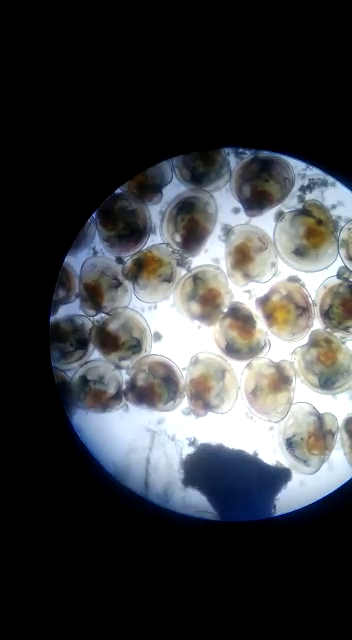
\includegraphics[width=0.68\textwidth]{2022_ConteoOstioncitos/figs/R0063.png}\\         
      \end{tabular}
\end{center}
\end{column} 
\end{columns} 


%\footnotetext[1]{\fullcite{MarcoNuno_ReporteTecnico2022_C}}
%\setcounter{footnote}{0}
%\footnotetext{\fullcite{MarcoNuno_ReporteTecnico2022_C}}
%\footfullcite{MarcoNuno_ReporteTecnico2022_C}
\footfullcite*{MarcoNuno_ReporteTecnico2022_C}
\end{frame}


\begin{frame}{\citetitle{MarcoNuno_ReporteTecnico2022_C} (2)}
\begin{columns}
\begin{column}{0.38\textwidth}
Problemas Encontrados:
\begin{itemize}
        \item Iluminación variable
        \item Ruido
	\end{itemize}
\textbf{Entrada}: Una secuencia de imágenes continua (video) en donde el técnico manipula la platina para abarcar un número de muestras mayor
\end{column}
\begin{column}{0.64\textwidth}  
\begin{center}
     \begin{tabular}{c}
         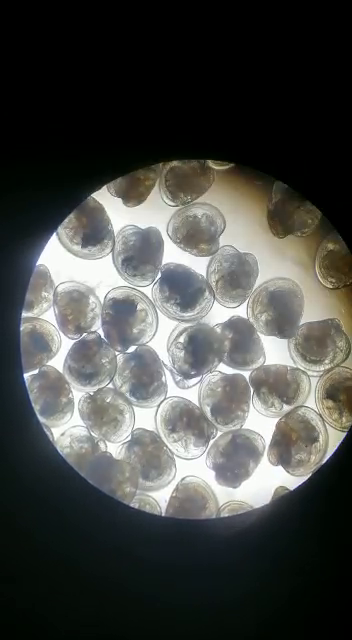
\includegraphics[width=0.24\textwidth]{2022_ConteoOstioncitos/figs/R0078.png}
         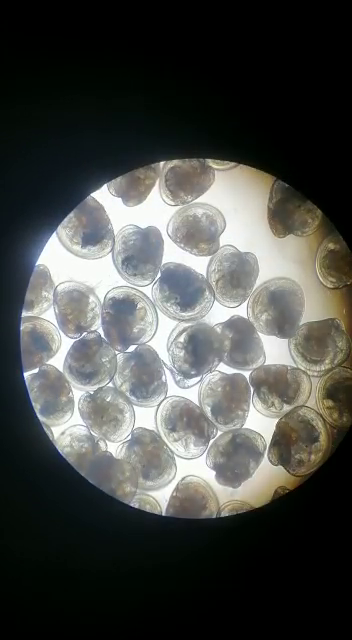
\includegraphics[width=0.24\textwidth]{2022_ConteoOstioncitos/figs/R0090.png}
         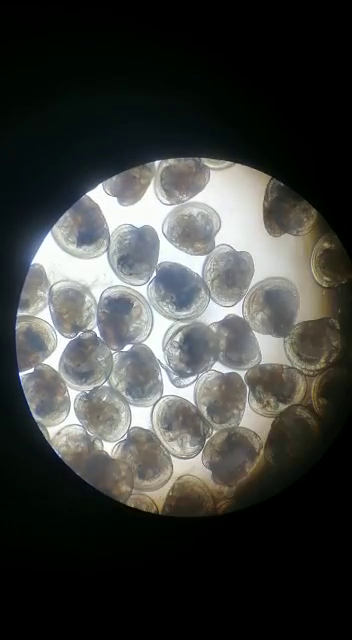
\includegraphics[width=0.24\textwidth]{2022_ConteoOstioncitos/figs/R0102.png}
         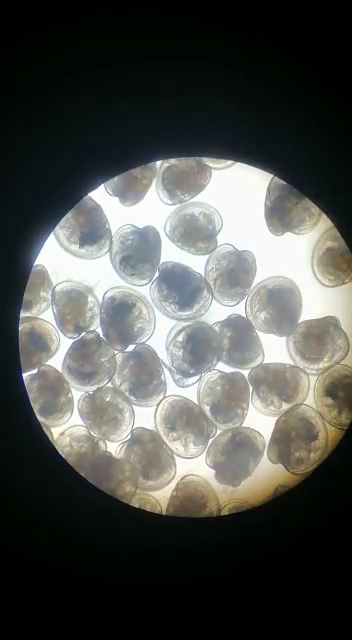
\includegraphics[width=0.24\textwidth]{2022_ConteoOstioncitos/figs/R0126.png}\\
          \end{tabular}
\end{center}
\end{column} 
\end{columns} 
\end{frame}

\begin{frame}{\citetitle{MarcoNuno_ReporteTecnico2022_C} (3)}



Etapas del algoritmo en desarrollo:
\begin{itemize}
        \item Encontrar los puntos característicos y los descriptores de caracteristícas, y estimar una correspondencia
        \item A partir de la correspondencia, estimar la matriz de Homografía y llevar a cabo transformación de tipo Warp para estimar el empalme de imágenes
	\end{itemize}

\begin{center}
 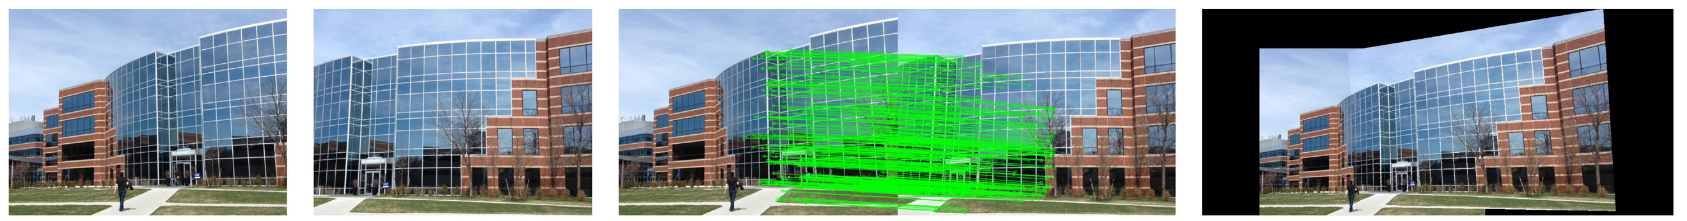
\includegraphics[width=0.95\textwidth]{2022_ConteoOstioncitos/figs/ImageMatchingAndRegistration.png}
\end{center}

\end{frame}


\begin{frame}{\citetitle{MarcoNuno_ReporteTecnico2022_C} (4)}
\begin{center}
 \begin{tabular}{c}
         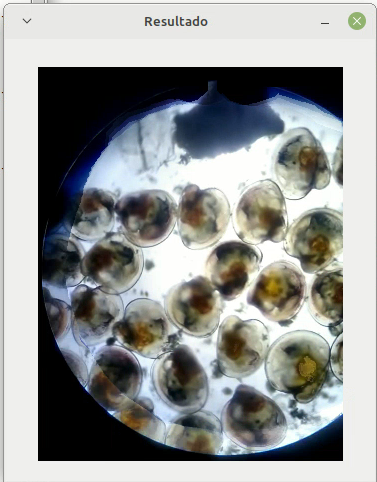
\includegraphics[width=0.24\textwidth]{2022_ConteoOstioncitos/figs/0049.png}
         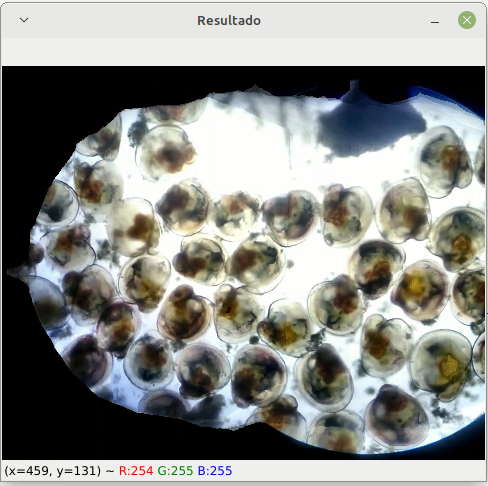
\includegraphics[width=0.24\textwidth]{2022_ConteoOstioncitos/figs/0085.png}
         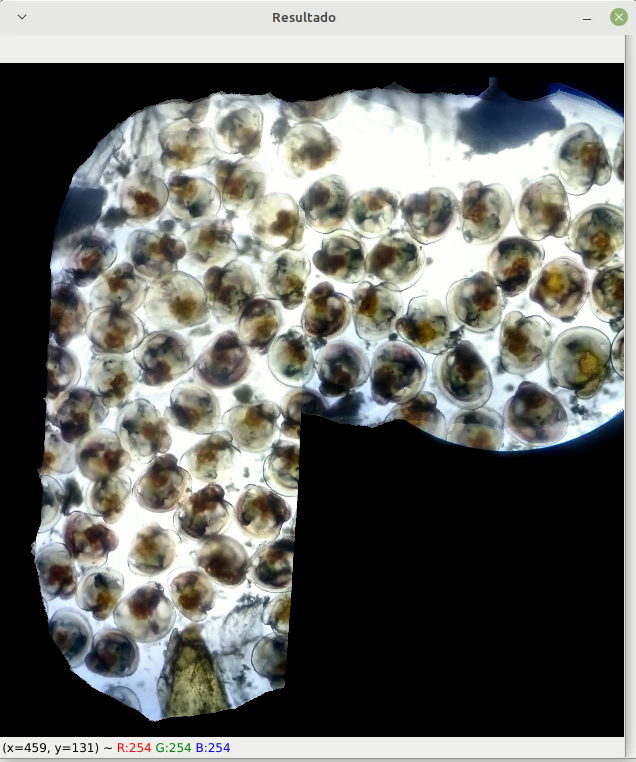
\includegraphics[width=0.24\textwidth]{2022_ConteoOstioncitos/figs/0193.png}
         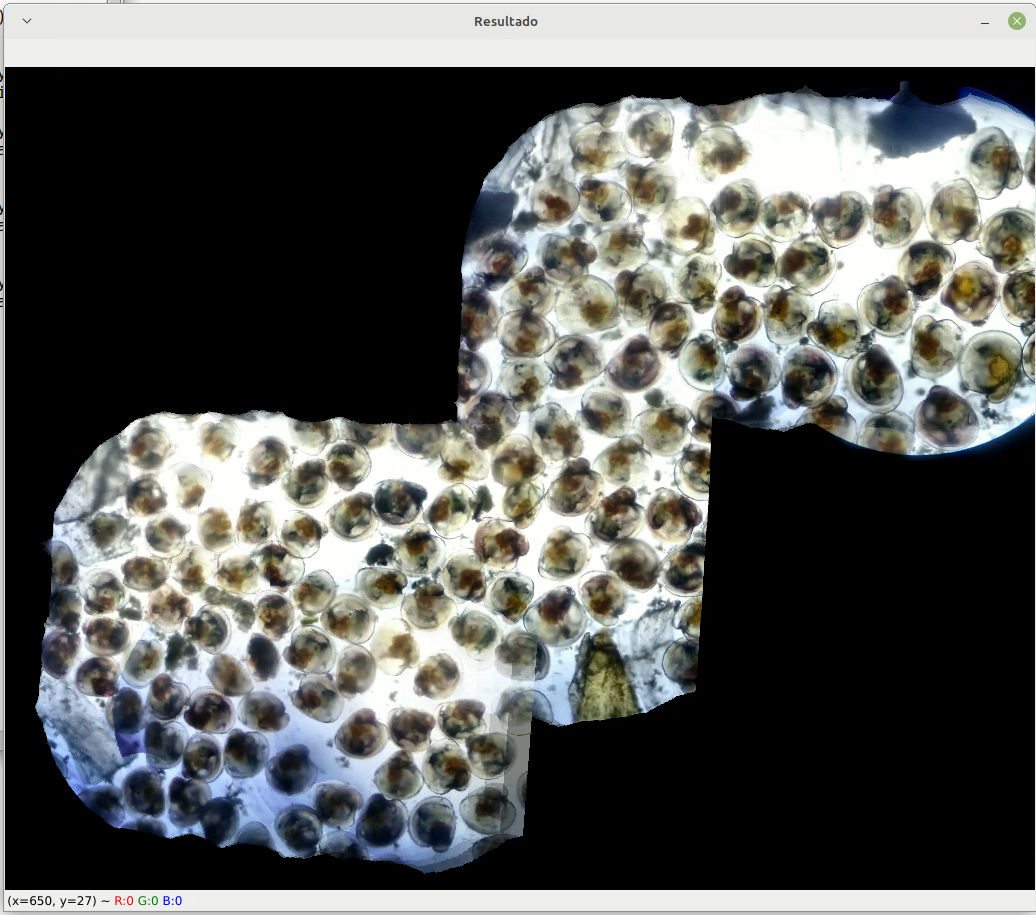
\includegraphics[width=0.24\textwidth]{2022_ConteoOstioncitos/figs/0373.png}\\
          \end{tabular}
\end{center}
\end{frame}



\begin{frame}{\citetitle{MarcoNuno_ReporteTecnico2022_C} (5)}
Resultado final de la generación del mosaico y del conteo de ostiones
\begin{center}
 \begin{tabular}{c}
         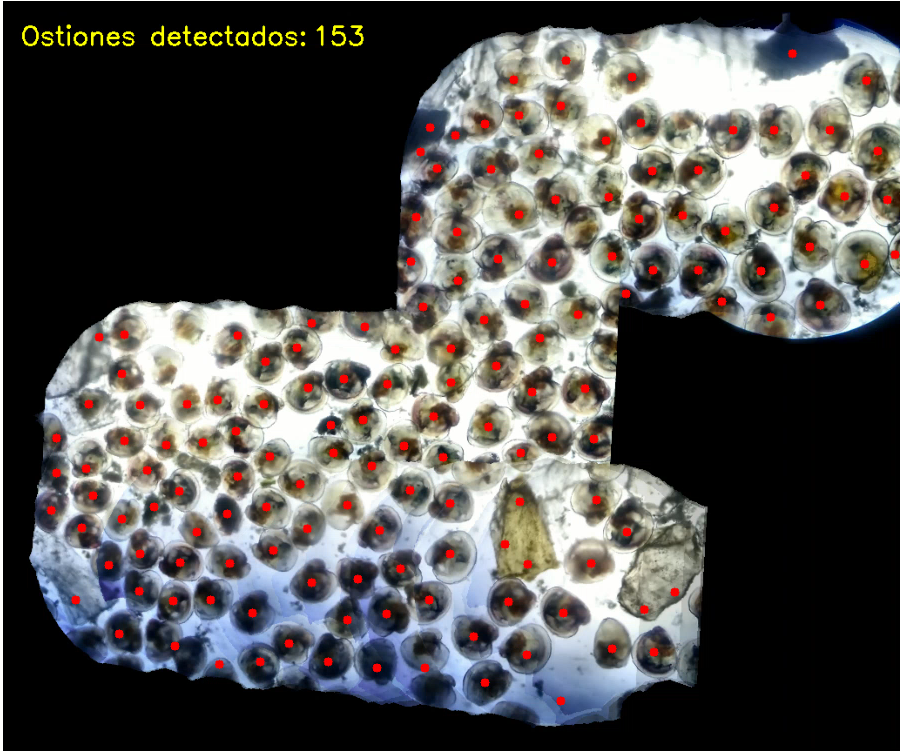
\includegraphics[width=0.50\textwidth]{2022_ConteoOstioncitos/figs/ConteoOstionesFinal.png}\\
          \end{tabular}
\end{center}

\end{frame}



\begin{frame}{\citetitle{MarcoNuno_ReporteTecnico2022_C} (6)}

\begin{itemize}
\item Hay un avance significativo con respecto al prototipo versión PC (cerca de completarse)
\begin{itemize} 
\item Se requieren más imágenes, que incluyan el conteo realizado de manera manual para contrastarlo con nuestros algoritmos
\item Posiblemente se deban afinar los algoritmos que se tienen desarrollados
\end{itemize}
\item Con respecto a la fase en el teléfono inteligente, se lleva un avance del 10\%, a reserva de la incorporación de un estudiante de estancia o estadía
\item Los resultados apuntan que es posible publicar los resultados en una Revista Indexada por el JCR
\end{itemize}




\end{frame}



